%!TEX root = ../thesis.tex
%*******************************************************************************
%****************************** Second Chapter *********************************
%*******************************************************************************

\chapter{Literature Review}

\ifpdf
    \graphicspath{{Chapter2/Figs/Raster/}{Chapter2/Figs/PDF/}{Chapter2/Figs/}}
\else
    \graphicspath{{Chapter2/Figs/Vector/}{Chapter2/Figs/}}
\fi
Statistical relational learning for knowledge graphs \newline
Latent feature models \newline
Link prediction

\section{Knowledge Graphs}
Knowledge graphs (KG) encode the relational information of a domain [reference]. KGs are composed of nodes and edges where nodes represent the entities and edges represent relations between entities. Two entities linked by a relation in a KG represents a fact, a KG is a collection of such facts represented as nodes and edges. Furthermore, the graphical structure of the representation models local, quasi-local and global properties about entities and relations. We can use direct entity relationships, or implicit structural properties to perform inference on the domain being modelled [reference]. For example %Start Trek graph 
\newline
KGs are modelled under closed world or open world assumptions [reference]. Under a closed world assumption, the KG is considered complete, and the graph completely captures all facts within a domain. Under an open world assumption, it is possible to infer new facts about a domain from existing facts [reference]. It is also possible to infer new facts about a domain from the structural properties of the graph. Under an open world assumption, link prediction is used to generate new facts from existing ones. Graphs can thus be queried for existing facts, and can be 'reason' new facts.
KGs have been applied to the field of information extraction [reference], search query augmentation [reference] and general question answering [reference].  \newline

Knowledge Bases \newline
Ontologies \newline
RDF \newline

% Uncomment this line, when you have siunitx package loaded.
%The SI Units for dynamic viscosity is \si{\newton\second\per\metre\squared}.
I'm going to randomly include a picture Figure~\ref{fig:minion}.


If you have trouble viewing this document contact Krishna at: \href{mailto:kks32@cam.ac.uk}{kks32@cam.ac.uk} or raise an issue at \url{https://github.com/kks32/phd-thesis-template/}


\begin{figure}[htbp!] 
\centering    
% 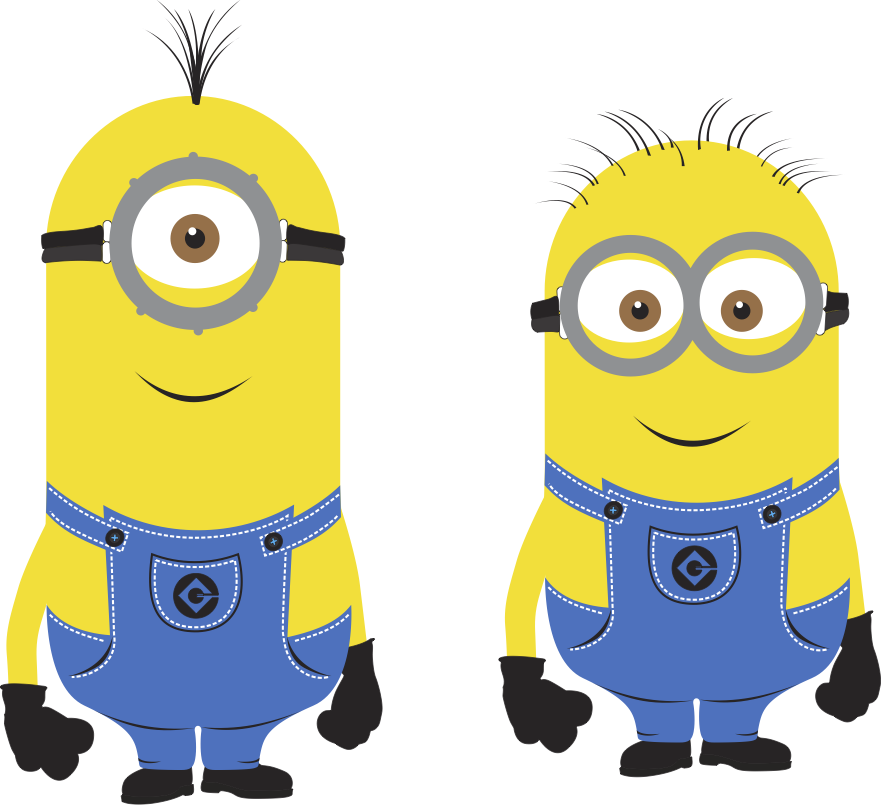
\includegraphics[width=1.0\textwidth]{minion}
\caption[Minion]{This is just a long figure caption for the minion in Despicable Me from Pixar}
\label{fig:minion}
\end{figure}


\section[Short title]{Matrix Factorization}
Singular Value Decomposition
Matrix factorisation is an approach used to compute latent features that capture relations between entities within a dataset [reference]. More formally, independent and identically distributed (IID) interactions between entities can be aggregated and represent in matrix format. The factorisation of the matrix will produce two real-valued unitary matrices that form a basis [reference], which can be thought of as a basis for a domain from where the data was sampled. Factorisation also produces a real-valued diagonal mastrix. The entries along the diagonal represent concepts captured by the dataset. A popular application of matrix factorisation is singular value decomposition [reference]. This is an implicit nodelling of relational domain concepts. \newline

\begin{enumerate}
\item The first topic is dull
\item The second topic is duller
\begin{enumerate}
\item The first subtopic is silly
\item The second subtopic is stupid
\end{enumerate}
\item The third topic is the dullest
\end{enumerate}

\section*{Itemize}
\begin{itemize}
\item The first topic is dull
\item The second topic is duller
\begin{itemize}
\item The first subtopic is silly
\item The second subtopic is stupid
\end{itemize}
\item The third topic is the dullest
\end{itemize}

\section*{Description}
\begin{description}
\item[The first topic] is dull
\item[The second topic] is duller
\begin{description}
\item[The first subtopic] is silly
\item[The second subtopic] is stupid
\end{description}
\item[The third topic] is the dullest
\end{description}


\clearpage

\section{Tensor Factorisation}
Tensor factorisation is an explicit modelling of entity relations using matrix slices of relational tensors [reference]. It involves modelling interactions of subject and object entities using relation-specific latent representations. These interactions have been modelled using the bilinlear tensor product, where the inner product of the subject entity is taken with a matrix relational representation, and the dot product of the generated embedding is then taken with the object entity. Bilinear tensor factorisation models are efficient in their number of parameters but lack expressiveness. Multilayer perceptrons were used to try overcome the lack of expressiveness however often suffer from overfitting. Recently convolutional neural networks have been proposed to allow expressive factorisation, do not suffer from overfitting and remain computationally efficient. \newline
Tensor factorisation is a technique used in latent feature modelling to build representations of entities modified by their relationships. These entity-relational representations are then combined with other entities to score facts within the KG as well as the possibility of a new fact. Tensor factorisation models aim to be linearly scalable with datasets and so attempt to balance expressiveness with parameter efficiency. \newline
RESCAL is a bilinear tensor model that combines latent entity-relational features of different entities using a matrix for each relation to compute a link score. \newline
Distmult simplifies RESCAL by limiting the full rank relational matrix to a diagonal, with zeros everywhere else. Relational transformation of the entity is thus limited only to a stretch, limiting the expressiveness of the model whilst improving scalability. \newline 
TransE projects object entities e2 via relation-specific offsets and then aggregates the generated embedding features with the subject entity e1 and uses the new representation as input to a scoring function. \newline

\section{Nonlinear Factorisation}
Parameterisation problem from tensor factorisation approach [nickel]. \newline
E-MLP ... \newline
ER-MLP ... \newline
Neural Tensor Networks extend the bilinear tensor product by concatenating the two entities and applying a weight operation on the concatenation to generate a latent representation which is then applied to a fully-connected neural layer to generation a score. HolE uses holographic embeddings described as circular correlations to compute triple scores. This involves taking the circular product of the interactions between each entity, and then taking the product of the generated representation along with a transposed relational vector. \newline
ComplEx ... \newline
HolE ... \newline
ConvE provides a more expressive model by taking the convolution of triple entities with a 2-dimensional convolutional relational model. This allows more expressive latent representations to be computed, whilst using a CNN architecture for parameter tying and parameter efficiency. \newline
HypER simplifies ConvE by using 1-dimensional convolutional relational filters. The convolution of the relational filter is then taken with the subject entity e1, before a dot product with the object entity e2 generates a triple score. \newline


\begin{landscape}

\section*{Subplots}
I can cite Wall-E (see Fig.~\ref{fig:WallE}) and Minions in despicable me (Fig.~\ref{fig:Minnion}) or I can cite the whole figure as Fig.~\ref{fig:animations}


\begin{figure}
  \centering
  \begin{subfigure}[b]{0.3\textwidth}
   %  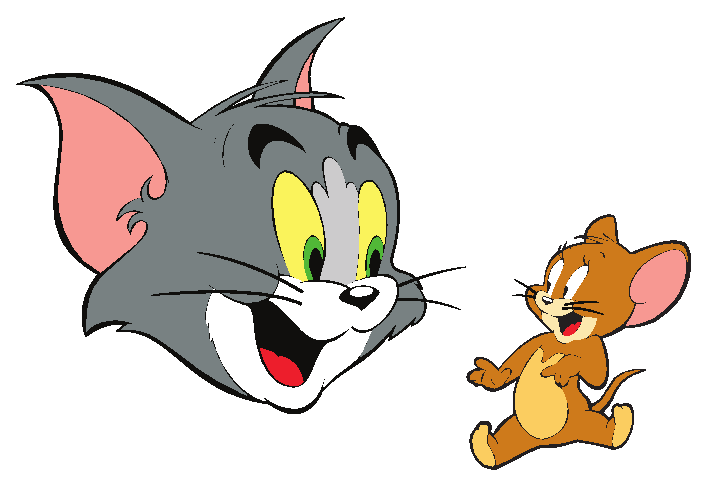
\includegraphics[width=\textwidth]{TomandJerry}
    \caption{Tom and Jerry}
    \label{fig:TomJerry}   
  \end{subfigure}             
  \begin{subfigure}[b]{0.3\textwidth}
   % 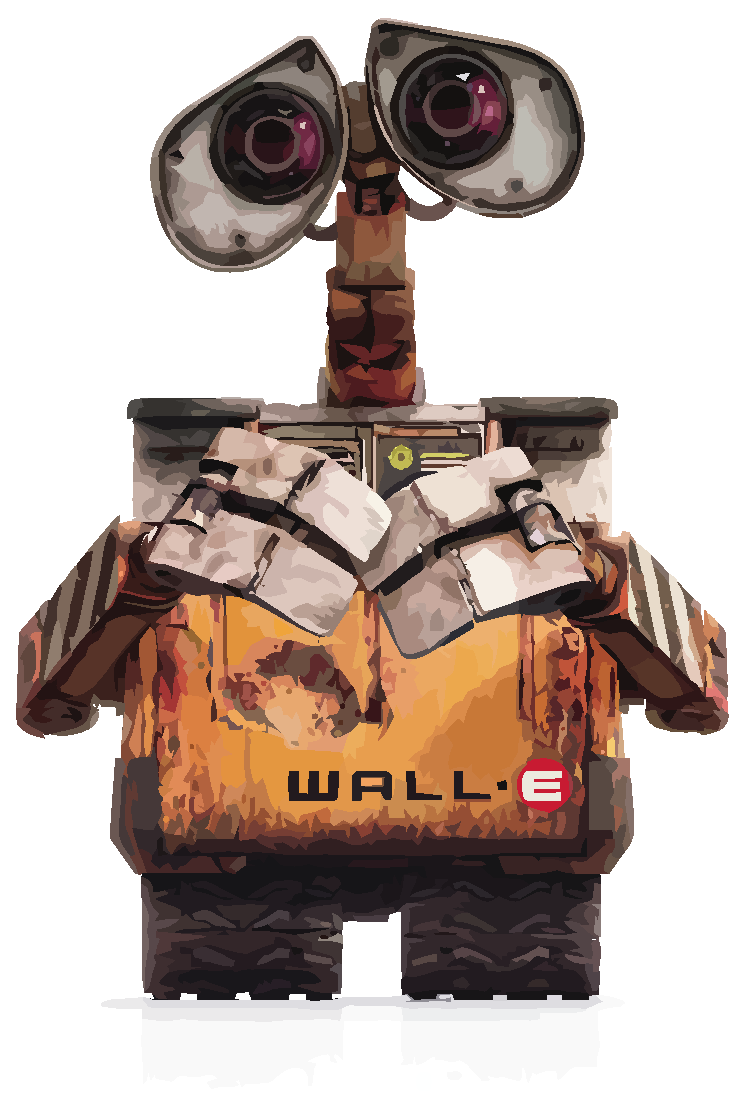
\includegraphics[width=\textwidth]{WallE}
    \caption{Wall-E}
    \label{fig:WallE}
  \end{subfigure}             
  \begin{subfigure}[b]{0.3\textwidth}
    %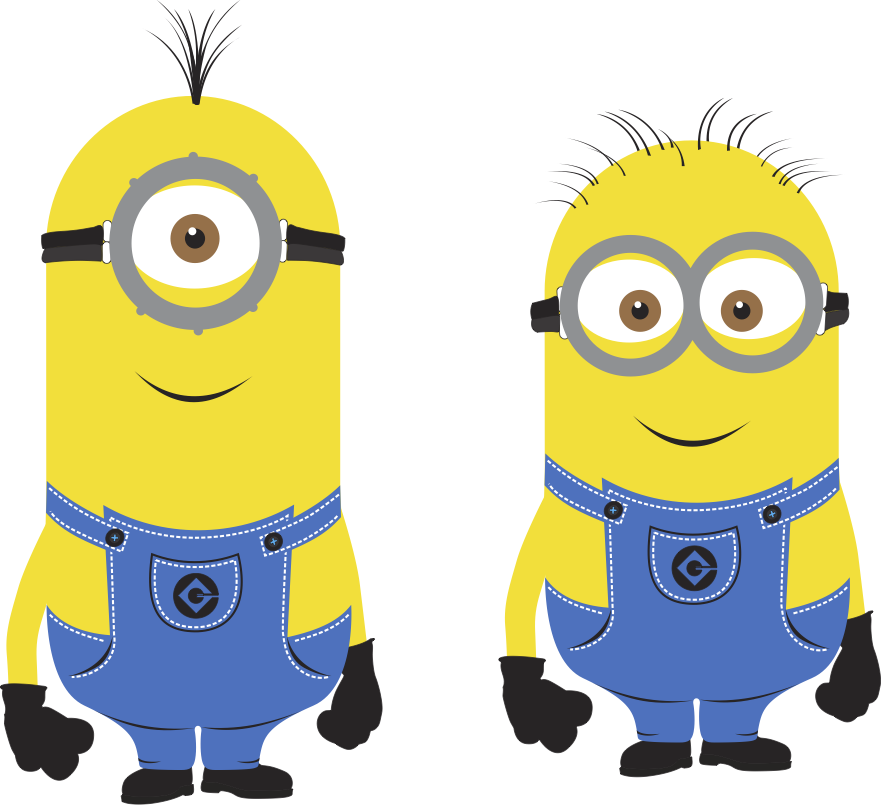
\includegraphics[width=\textwidth]{minion}
    \caption{Minions}
    \label{fig:Minnion}
  \end{subfigure}
  \caption{Best Animations}
  \label{fig:animations}
\end{figure}


\end{landscape}
